\documentclass[UTF8]{ctexart}
\usepackage[a4paper,margin=2.4cm]{geometry}
\usepackage{amsmath,amssymb,mathtools}
\usepackage{graphicx}
\usepackage{booktabs}
\usepackage{hyperref}

\title{第三题：兴奋-抑制神经网络的 Hopf 分叉分析与数值验证}
\author{}
\date{\today}

\begin{document}
\emergencystretch=2em
\maketitle

\section{模型与目标}

题目给出的兴奋-抑制神经网络模型为
\begin{align}
\tau_E\frac{dv_E}{dt}
&=-v_E+\bigl[M_{EE}v_E-M_{EI}v_I+h_E\bigr]_+,
\label{eq:model_e}\\
\tau_I\frac{dv_I}{dt}
&=-v_I+\bigl[M_{IE}v_E-M_{II}v_I+h_I\bigr]_+,
\label{eq:model_i}
\end{align}
其中
\[
[z]_+=\max\{z,0\}.
\]
$v_E,v_I$ 分别表示兴奋性和抑制性神经元群发放率，$M_{ab}$ 为连接权重，
$h_E,h_I$ 为外部输入。题目要求分别对参数 $\tau_I$ 和 $h_E$ 做 Hopf 分叉分析，
并用数值模拟验证。

由于模型使用 ReLU 非线性，它是分段线性系统。在任意一个固定活动区中，右端关于
$(v_E,v_I)$ 是线性的；当平衡点落在双活动区，即两个 ReLU 括号内都为正时，可以进行
通常的局部线性化分析。若平衡点穿越 ReLU 的折点边界，则发生的是非光滑的边界切换，
不属于经典光滑 Hopf 分叉。

\section{双活动区中的平衡点}

在双活动区中有
\[
M_{EE}v_E-M_{EI}v_I+h_E>0,\qquad
M_{IE}v_E-M_{II}v_I+h_I>0.
\]
此时模型化为线性仿射系统
\begin{align}
\tau_E\dot v_E
&=(M_{EE}-1)v_E-M_{EI}v_I+h_E,\\
\tau_I\dot v_I
&=M_{IE}v_E-(M_{II}+1)v_I+h_I.
\end{align}
令
\[
a=M_{EE}-1,\qquad b=-M_{EI},\qquad
c=M_{IE},\qquad d=-(M_{II}+1).
\]
平衡点满足
\[
\begin{pmatrix}
a & b\\
c & d
\end{pmatrix}
\begin{pmatrix}
v_E^*\\v_I^*
\end{pmatrix}
=
\begin{pmatrix}
-h_E\\-h_I
\end{pmatrix}.
\]
矩阵行列式为
\[
K=ad-bc=M_{EI}M_{IE}-(M_{EE}-1)(M_{II}+1).
\]
若 $K\ne0$，则双活动区候选平衡点为
\begin{align}
v_E^*
&=\frac{(M_{II}+1)h_E-M_{EI}h_I}{K},
\label{eq:eq_ve}\\
v_I^*
&=\frac{M_{IE}h_E-(M_{EE}-1)h_I}{K}.
\label{eq:eq_vi}
\end{align}
该平衡点真正属于双活动区，需要
\[
v_E^*>0,\qquad v_I^*>0.
\]
在 $K>0$ 且 $h_I>0$ 的常见情形下，这等价于
\begin{equation}
h_E>
\max\left\{
\frac{M_{EI}h_I}{M_{II}+1},
\frac{(M_{EE}-1)h_I}{M_{IE}}
\right\}.
\label{eq:active_boundary}
\end{equation}

\section{参数 tau\_I 的 Hopf 分叉分析}

在双活动区中，系统在平衡点处的雅可比矩阵为
\begin{equation}
J=
\begin{pmatrix}
\dfrac{M_{EE}-1}{\tau_E} & -\dfrac{M_{EI}}{\tau_E}\\[8pt]
\dfrac{M_{IE}}{\tau_I} & -\dfrac{M_{II}+1}{\tau_I}
\end{pmatrix}.
\label{eq:jacobian}
\end{equation}
记迹和行列式分别为
\begin{align}
T(\tau_I)
&=\operatorname{tr}J
=\frac{M_{EE}-1}{\tau_E}-\frac{M_{II}+1}{\tau_I},
\label{eq:trace}\\
D(\tau_I)
&=\det J
=\frac{M_{EI}M_{IE}-(M_{EE}-1)(M_{II}+1)}
{\tau_E\tau_I}
=\frac{K}{\tau_E\tau_I}.
\label{eq:det}
\end{align}
二维系统发生 Hopf 分叉的线性条件为
\[
T(\tau_I^H)=0,\qquad D(\tau_I^H)>0,
\]
并且特征值实部要横截穿过虚轴。由 \eqref{eq:trace} 得
\begin{equation}
\tau_I^H
=\tau_E\frac{M_{II}+1}{M_{EE}-1}.
\label{eq:tau_hopf}
\end{equation}
因此需要
\[
M_{EE}>1,\qquad K>0.
\]
此时 Hopf 点处的特征值为
\[
\lambda_{1,2}=\pm i\omega_H,\qquad
\omega_H=\sqrt{D(\tau_I^H)}
=\sqrt{\frac{K}{\tau_E\tau_I^H}}.
\]
横截条件为
\[
\frac{dT}{d\tau_I}
=\frac{M_{II}+1}{\tau_I^2}>0,
\]
所以当 $\tau_I$ 增大并穿过 $\tau_I^H$ 时，特征值实部由负变正，平衡点由稳定焦点变为
不稳定焦点。

需要注意的是，给定模型是精确分段线性的 ReLU 系统。在平衡点附近且仍处于双活动区时，
非线性高阶项为零，因此严格的光滑 Hopf 正规形一阶 Lyapunov 系数退化。数值中观察到的
稳定振荡不是由局部三次项饱和产生，而是轨道离开双活动线性区后受到 ReLU 边界的非光滑
限制而形成。因此本文将其称为 ReLU 分段线性系统中的 Hopf 型失稳和边界饱和振荡。

\section{参数 h\_E 的 Hopf 分叉分析}

由 \eqref{eq:eq_ve}--\eqref{eq:eq_vi} 可知，$h_E$ 会改变平衡点位置；但是由
\eqref{eq:jacobian}--\eqref{eq:det} 可知，在固定活动区内雅可比矩阵、迹和行列式都不含
$h_E$。因此，在双活动区内部改变 $h_E$ 时，
\[
\frac{\partial T}{\partial h_E}=0,\qquad
\frac{\partial D}{\partial h_E}=0,
\]
特征值不会随 $h_E$ 移动，也就不可能通过 $h_E$ 产生经典 Hopf 分叉。

$h_E$ 的作用是移动平衡点，并可能使平衡点穿过 ReLU 活动边界 \eqref{eq:active_boundary}。
这种现象是非光滑边界切换或边界碰撞，而不是 Hopf 分叉。若把 ReLU 换成光滑 Sigmoid
或光滑化 ReLU，则 $h_E$ 会改变平衡点所在位置处的增益，从而可能间接影响雅可比矩阵；
但对题目给出的精确 $[z]_+$ 模型，$h_E$ 在同一线性区中不触发 Hopf。

\section{数值模拟方法}

程序文件为 \texttt{e\_i\_hopf\_sim.py}。数值积分使用四阶 Runge--Kutta 方法。为了清楚验证
理论结论，取参数
\[
\tau_E=1,\quad M_{EE}=2,\quad M_{EI}=1.5,\quad
M_{IE}=2,\quad M_{II}=1,\quad h_E=0.25,\quad h_I=0.20.
\]
此时
\[
K=1,\qquad
\tau_I^H=2,\qquad
\omega_H=\sqrt{\frac{1}{2}}\approx0.7071.
\]
平衡点为
\[
(v_E^*,v_I^*)=(0.2,0.3),
\]
并且满足双活动区条件。对 $h_E$ 而言，双活动区边界为
\[
h_E>\max\left\{\frac{1.5\times0.2}{2},\frac{1\times0.2}{2}\right\}=0.15.
\]

运行命令为
\[
\texttt{python e\_i\_hopf\_sim.py}.
\]
程序输出 $\tau_I$ 扫描、$h_E$ 扫描、时间序列和相图。扫描中振幅定义为去掉前
$55\%$ 暂态后 $v_E$ 的最大值减最小值。

\section{数值结果与解释}

\subsection{tau\_I 扫描}

\begin{figure}[htbp]
\centering
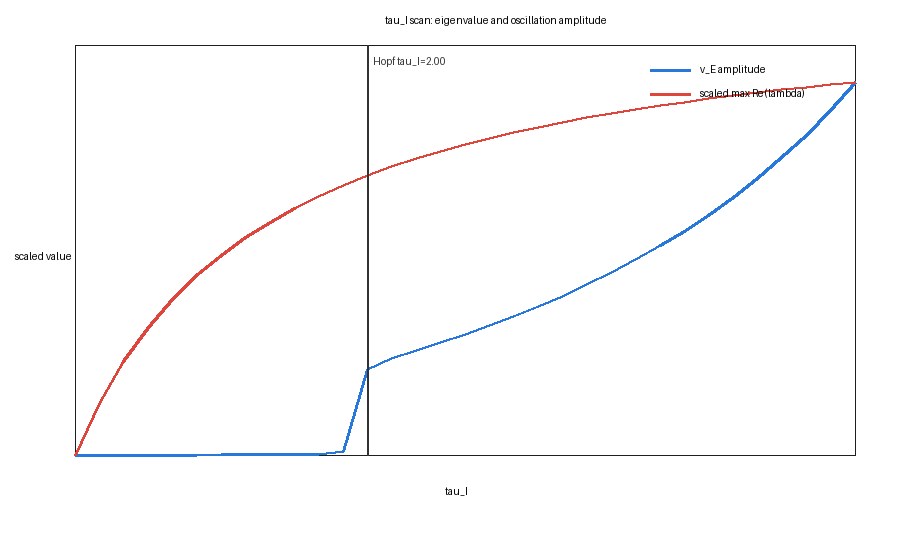
\includegraphics[width=0.86\linewidth]{results/tau_i_scan.png}
\caption{$\tau_I$ 扫描：特征值实部穿越与振荡振幅}
\label{fig:tau_scan}
\end{figure}

图 \ref{fig:tau_scan} 中黑色竖线为理论 Hopf 点 $\tau_I^H=2$。红线为缩放后的最大特征值实部，
蓝线为数值积分得到的 $v_E$ 振荡振幅。可以看到，当 $\tau_I<2$ 时，特征值实部为负，
轨道收敛到平衡点，振幅近似为零；当 $\tau_I>2$ 后，特征值实部为正，平衡点失稳，
轨道进入由 ReLU 边界限制的持续振荡。数值结果与 \eqref{eq:tau_hopf} 的理论临界值一致。

\begin{figure}[htbp]
\centering
\begin{minipage}{0.48\linewidth}
\centering
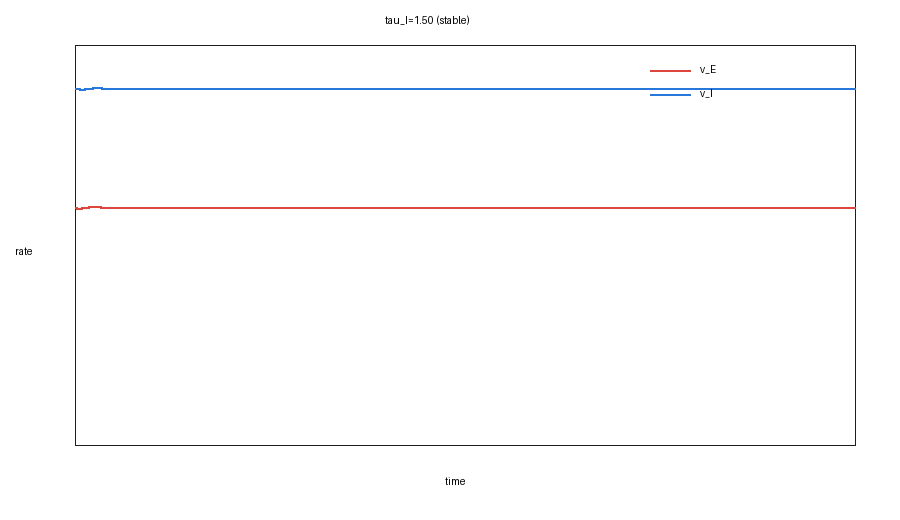
\includegraphics[width=\linewidth]{results/time_series_tau_stable.png}
\caption{$\tau_I=1.5$ 时的稳定时间序列}
\label{fig:stable_ts}
\end{minipage}
\hfill
\begin{minipage}{0.48\linewidth}
\centering
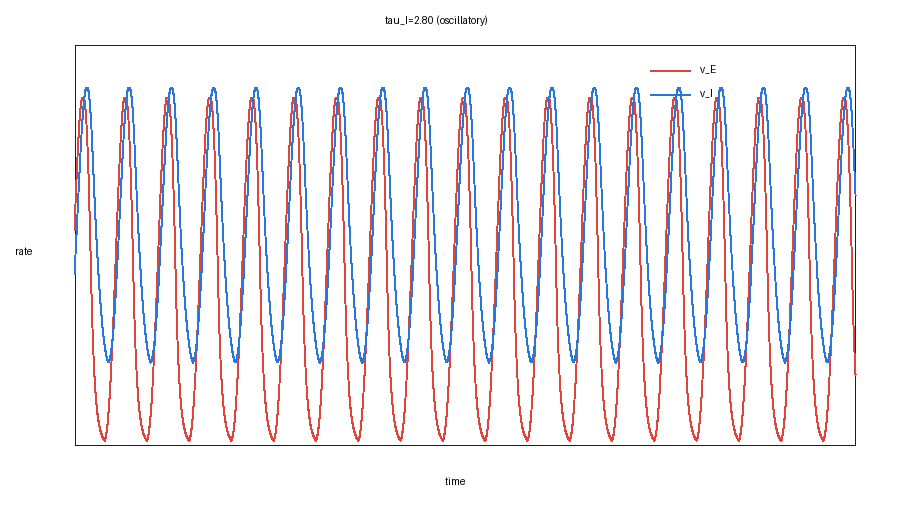
\includegraphics[width=\linewidth]{results/time_series_tau_oscillatory.png}
\caption{$\tau_I=2.8$ 时的振荡时间序列}
\label{fig:osc_ts}
\end{minipage}
\end{figure}

图 \ref{fig:stable_ts} 和图 \ref{fig:osc_ts} 更直接展示了分叉前后的动力学差异。
$\tau_I=1.5$ 时，
\[
T=1-\frac{2}{1.5}=-\frac13<0,
\]
平衡点是稳定焦点，兴奋性和抑制性发放率最终趋于常数。$\tau_I=2.8$ 时，
\[
T=1-\frac{2}{2.8}>0,
\]
平衡点失稳，兴奋群和抑制群交替升降，形成稳定周期振荡。抑制群相对兴奋群有相位滞后，
这符合 E-I 反馈环中兴奋驱动抑制、抑制再压低兴奋的机制。

\begin{figure}[htbp]
\centering
\begin{minipage}{0.48\linewidth}
\centering
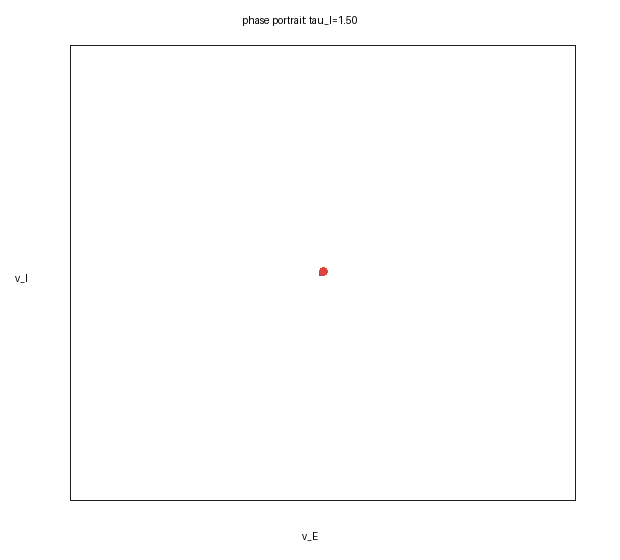
\includegraphics[width=\linewidth]{results/phase_tau_stable.png}
\caption{$\tau_I=1.5$ 的相图}
\label{fig:stable_phase}
\end{minipage}
\hfill
\begin{minipage}{0.48\linewidth}
\centering
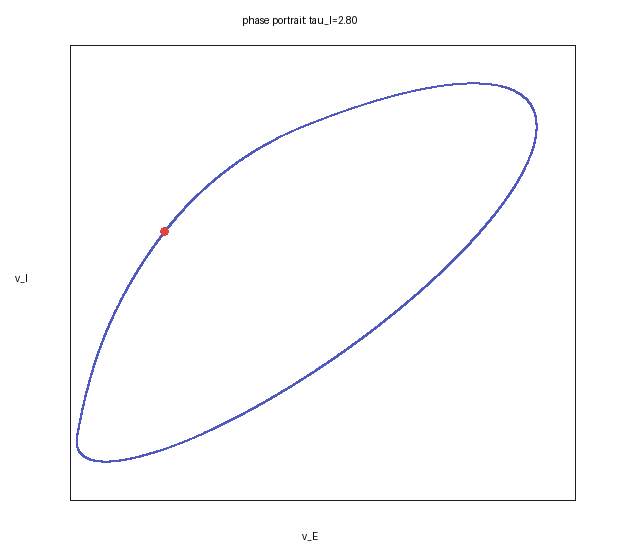
\includegraphics[width=\linewidth]{results/phase_tau_oscillatory.png}
\caption{$\tau_I=2.8$ 的相图}
\label{fig:osc_phase}
\end{minipage}
\end{figure}

相图进一步说明：分叉前轨道螺旋收敛到平衡点；分叉后轨道围绕平衡点运动，并在 ReLU
分段边界作用下形成闭合环。由于模型是分段线性的，闭合环的幅值不是由局部三阶非线性决定，
而是由全局分段结构决定。

\subsection{h\_E 扫描}

\begin{figure}[htbp]
\centering
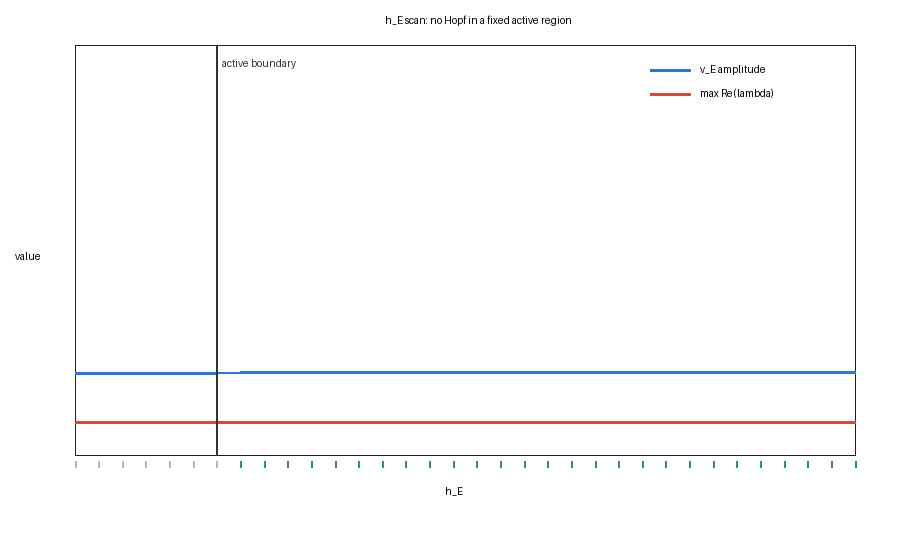
\includegraphics[width=0.86\linewidth]{results/h_e_scan.png}
\caption{$h_E$ 扫描：固定活动区内无 Hopf 分叉}
\label{fig:h_scan}
\end{figure}

图 \ref{fig:h_scan} 固定 $\tau_I=1.5$，扫描 $h_E$。黑色竖线是双活动区边界
$h_E=0.15$；底部绿色短线表示候选平衡点位于双活动区。红线为最大特征值实部，
其值始终为
\[
\frac12 T=\frac12\left(1-\frac{2}{1.5}\right)=-\frac16,
\]
不随 $h_E$ 变化。蓝线表示数值振幅，也基本为零。由此验证了理论结论：
在题目给出的 ReLU 模型中，$h_E$ 只移动平衡点和改变活动区归属，不会让一对复特征值
随 $h_E$ 穿过虚轴，因此不存在由 $h_E$ 诱导的经典 Hopf 分叉。

\section{结论}

在双活动区中，E-I 网络的 Hopf 条件由雅可比矩阵迹和行列式给出：
\[
\tau_I^H=\tau_E\frac{M_{II}+1}{M_{EE}-1},\qquad
K=M_{EI}M_{IE}-(M_{EE}-1)(M_{II}+1)>0.
\]
当 $\tau_I$ 增大穿过 $\tau_I^H$ 时，平衡点从稳定焦点变为不稳定焦点，数值模拟显示
系统进入由 ReLU 边界限制的持续振荡。对于 $h_E$，它不进入固定活动区内的雅可比矩阵，
所以不能产生经典 Hopf 分叉；它只能通过移动平衡点导致活动区切换。数值扫描与这一分析一致。

\end{document}
